\documentclass[a4paper,10pt]{article}

\usepackage{fontspec}
\usepackage[T1]{fontenc}
\usepackage{geometry}
\usepackage{xcolor}
\usepackage{graphicx}
\usepackage{tabularx}
\usepackage[hidelinks]{hyperref}
\usepackage{array}
\usepackage{ragged2e}

\geometry{left=1.25cm, top=0.75cm, right=1.1cm, bottom=0.75cm}
\pagestyle{empty}
\urlstyle{same}
\setlength{\tabcolsep}{0pt}
\setlength{\parindent}{0pt}
\setlength{\parskip}{0pt}
\setmainfont{Times New Roman}
\newfontfamily\zhfont{Songti SC}
\XeTeXlinebreaklocale "zh"
\XeTeXlinebreakskip=0pt plus 1pt
\renewcommand{\arraystretch}{1.06}
\renewcommand{\labelitemi}{$\vcenter{\hbox{\tiny$\bullet$}}$}

\newcolumntype{L}{>{\raggedright\arraybackslash}X}
\newcolumntype{R}{>{\raggedleft\arraybackslash}X}

\newcommand{\cvsection}[1]{%
  \vspace{1.2mm}
  {\large\bfseries #1}\\[-1mm]
  {\color{black}\rule{\textwidth}{0.4pt}}
  \vspace{0.2mm}
}

\newcommand{\resumeSubheading}[4]{
  \vspace{0.2mm}\item
  \begin{tabular*}{0.98\textwidth}[t]{l@{\extracolsep{\fill}}r}
    \textbf{#1} & \textit{\footnotesize #4} \\
    \footnotesize #3 & \footnotesize #2
  \end{tabular*}
  \vspace{0mm}
}

\newcommand{\resumeProject}[4]{
  \vspace{0.2mm}\item
  \begin{tabular*}{0.98\textwidth}[t]{l@{\extracolsep{\fill}}r}
    \textbf{#1} & \textit{\footnotesize #3} \\
    \footnotesize\textit{#2} & \footnotesize #4
  \end{tabular*}
  \vspace{0mm}
}

\newcommand{\resumePOR}[3]{
  \vspace{0.1mm}\item
  \begin{tabular*}{0.97\textwidth}[t]{l@{\extracolsep{\fill}}r}
    \textbf{#1}\hspace{0.3mm}#2 & \textit{\small #3}
  \end{tabular*}
  \vspace{0mm}
}

\newcommand{\resumeSubHeadingListStart}{\begin{itemize}\setlength{\itemsep}{0mm}\setlength{\parsep}{0pt}\setlength{\topsep}{0.2mm}}
\newcommand{\resumeSubHeadingListEnd}{\end{itemize}\vspace{-1.0mm}}
\newcommand{\resumeItemListStart}{\begin{itemize}\small\setlength{\itemsep}{0mm}\setlength{\parsep}{0pt}\setlength{\topsep}{0mm}}
\newcommand{\resumeItemListEnd}{\end{itemize}\vspace{-1.2mm}}

\newcommand{\name}{管进程 \, / \, Jincheng Guan}
\newcommand{\phone}{15345462557}
\newcommand{\email}{guanjincheng@mail.ustc.edu.cn}
\newcommand{\github}{https://github.com/gjc2}
\newcommand{\homepage}{https://gjc2.github.io}

\begin{document}
\zhfont
\pagecolor{white}
\fontsize{9.4pt}{10.7pt}\selectfont

\begin{minipage}[t]{2.55cm}
  \vspace{0pt}
  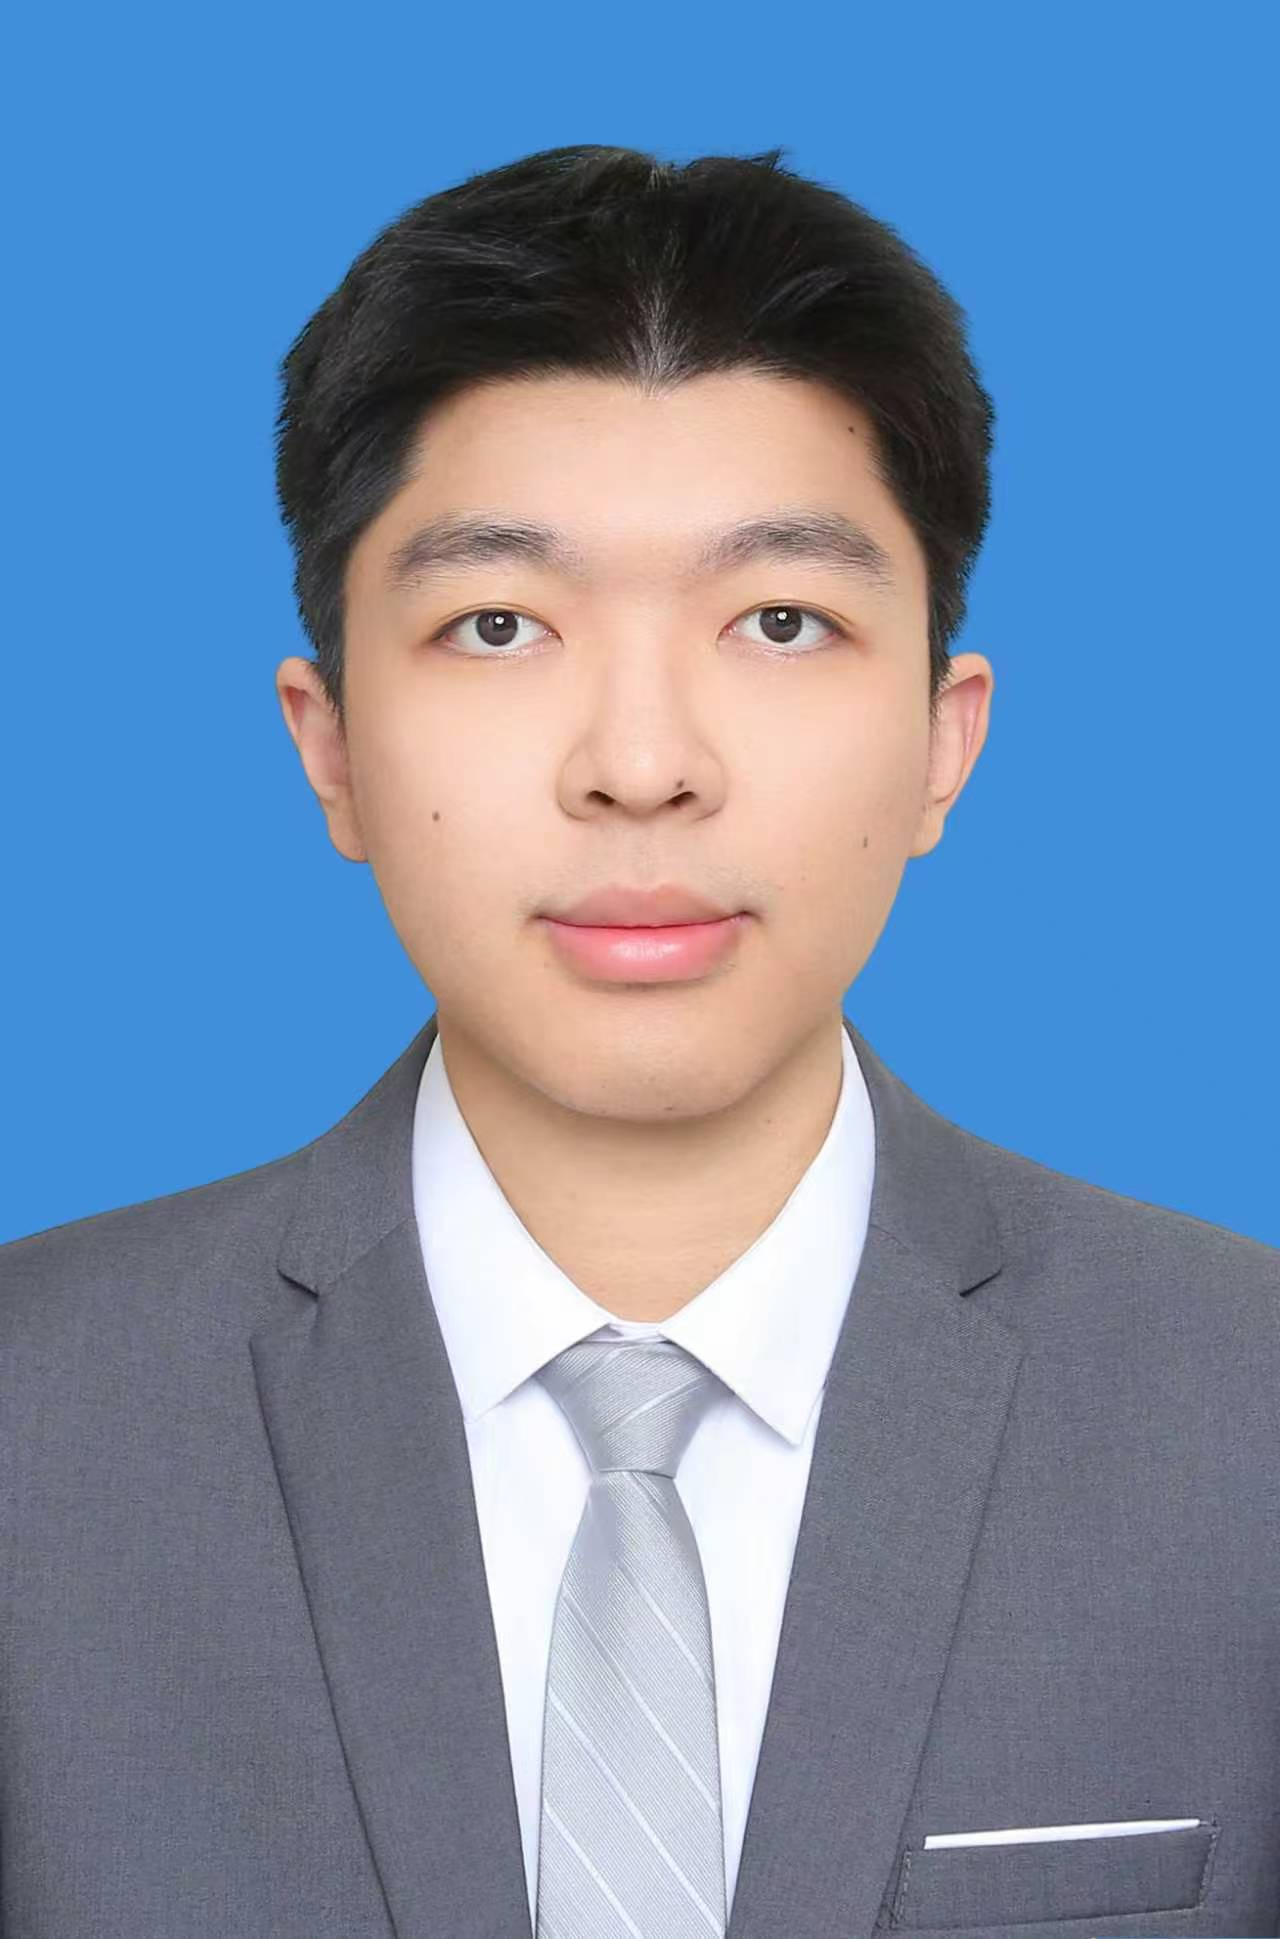
\includegraphics[width=2.25cm,height=3.0cm,keepaspectratio]{id_photo.jpg}
\end{minipage}
\hfill
\begin{minipage}[t]{\dimexpr\linewidth-2.85cm\relax}
  \vspace{0pt}
  {\LARGE\bfseries \name}\\[1.5mm]
  中国科学技术大学（USTC）计算机科学与技术学院 \hfill +86-\phone\\
  硕士研究生，计算机科学与技术 \hfill \href{mailto:\email}{\email}\\
  导师：\href{http://staff.ustc.edu.cn/~wwwucuc/}{邵帅 教授} \hfill \href{\homepage}{\homepage}\\
  研究兴趣：Counting Complexity；Holant；Edge CSP；判定与优化问题
\end{minipage}

\vspace{1mm}

\cvsection{教育经历}
\resumeSubHeadingListStart
  \resumeSubheading
    {中国科学技术大学}{}
    {计算机科学与技术学院，计算机科学与技术，硕士研究生；导师：\href{http://staff.ustc.edu.cn/~wwwucuc/}{邵帅 教授}}
    {2024--至今}
  \resumeSubheading
    {山东大学}{GPA: 90.17/100 \quad Rank: 4/18}
    {计算机科学与技术学院，泰山学堂（计算机），工学学士}
    {2020--2024}
\resumeSubHeadingListEnd
\vspace{0mm}

\cvsection{个人介绍}
\small{
我是中国科学技术大学计算机科学与技术学院二年级硕士生，导师为邵帅教授。本科毕业于山东大学计算机科学与技术学院泰山学堂（计算机）。我的研究兴趣主要在理论计算机科学，尤其关注 counting complexity 中的 Holant 问题，以及 Holant 或 edge CSP 框架下判定问题和优化问题的复杂性分类。
}

\vspace{1mm}

\cvsection{科研经历}
\resumeSubHeadingListStart
  \resumeSubheading
    {中国科学技术大学，理论计算机科学方向}{}
    {导师：\href{http://staff.ustc.edu.cn/~wwwucuc/}{邵帅 教授}}
    {2024--至今}
    \vspace{-1mm}
    \resumeItemListStart
      \item 关注 counting complexity 与 Holant 问题中的复杂性分类、tractability/hardness 划分等主题。
      \item 研究 Holant 或 edge CSP 框架下的判定问题与优化问题。
    \resumeItemListEnd

  \resumeSubheading
    {山东大学 智能算法与软件实验室}{}
    {参数算法、近似算法与图算法方向}
    {2021--2023}
    \vspace{-1mm}
    \resumeItemListStart
      \item 学习并参与图论上的参数算法和近似算法相关问题。
      \item 参与图的直径缩减问题相关讨论与研究训练。
    \resumeItemListEnd

  \resumeSubheading
    {山东大学 ACM 实验室}{}
    {程序设计竞赛与算法训练}
    {2020--2022}
    \vspace{-1mm}
    \resumeItemListStart
      \item 获 2021 年青岛市大学生 ACM 程序设计竞赛银奖。
      \item 获 2022 年山东大学“极客出发”ACM 赛道二等奖，2023 年山东大学“极客出发”ACM 赛道第二名。
    \resumeItemListEnd
\resumeSubHeadingListEnd
\vspace{0mm}

\cvsection{项目经历}
\resumeSubHeadingListStart
  \resumeProject
    {数据库 OJ 系统}
    {数据库课程设计：实现可进行 SQL 在线判题的 OJ 系统}
    {2023.05}
    {}
    \resumeItemListStart
      \item 技术栈：MySQL、Flask、Jinja2、Bootstrap、jQuery UI、CodeMirror。
      \item 实现题目提交验证、题目搜索、常用表查询等基本功能，并扩展评论区、用户信息界面等功能。
    \resumeItemListEnd

  \resumeProject
    {PL/0 编译器}
    {编译原理课程设计：实现 PL/0 语言编译器}
    {2022.12}
    {}
    \resumeItemListStart
      \item 使用 LR(0) 自底向上的语法分析流程，完成语义分析和目标代码生成。
      \item 使用 C++ 实现，注重模块化封装与代码结构清晰性。
    \resumeItemListEnd
\resumeSubHeadingListEnd
\vspace{0mm}

\cvsection{个人能力}
\small{
  \textbf{英语能力}{：CET-4 521；CET-6 503} \\
  \textbf{编程能力}{：2023 CCF CSP 认证 300 分（Top 3.33\%）} \\
  \textbf{编程语言}{：C、C++、Python、Matlab、汇编} \\
  \textbf{工具与框架}{：Flask、PyTorch、MySQL、\LaTeX}
}
\vspace{0mm}

\cvsection{荣誉奖项}
\small
\begin{tabular*}{\textwidth}{l@{\extracolsep{\fill}}r}
山东大学三好学生，前 5\% & 2021.12 \\
山东大学学业一等奖学金，前 5\% & 2021.12 \\
山东大学玲珑集团奖学金，前 5\% & 2021.12 \\
全国大学生数学建模竞赛省一等奖，前 10\% & 2022.11 \\
全国高中数学奥林匹克竞赛省级赛区一等奖 & 2019
\end{tabular*}

\end{document}
